% GENERATED by paper/ijdc/build_tex.py from paper/manuscript.md - do not edit by hand.
\documentclass[lineno,12pt]{sn-jnl}% IJDC template: Math and Physical Sciences Reference Style
\usepackage{cite}%
\usepackage{graphicx}%
\usepackage{multirow}%
\usepackage{amsmath,amssymb,amsfonts}%
\usepackage{amsthm}%
\usepackage{mathrsfs}%
\usepackage[title]{appendix}%
\usepackage{xcolor}%
\usepackage{textcomp}%
\usepackage{manyfoot}%
\usepackage{booktabs}%
\usepackage{bm}%
\usepackage{array}%
\graphicspath{{../figures/}{figures/}}
\providecommand{\tightlist}{\setlength{\itemsep}{0pt}\setlength{\parskip}{0pt}}
\theoremstyle{thmstyleone}%
\newtheorem{proposition}{Proposition}%
\raggedbottom
\begin{document}
\title[Prediction-augmented, payload-wind-aware multiple-observer control]{Prediction-augmented, payload-wind-aware multiple-observer control of a quadrotor with a slung load in measured wind}

\abstract{A quadrotor carrying a load on a cable in wind is disturbed by the cable force of the swinging load and by the wind on the airframe and on the load. Observer-based anti-disturbance controllers estimate both and cancel the estimates. This paper argues that, once the wind is measured, the remaining error is set by two gaps in the controller's model rather than by the quality of the estimates: the loop delay acts on a payload force that is periodic along a planned trajectory, and the wind feed-forward omits the drag on the load. Both gaps are closed with knowledge the controller already holds: the payload estimate is propagated over the loop delay through the observer's own exosystem, and the measured-wind feed-forward is scaled by the share of the wind force that the force balance of the coupled system assigns to the load. The resulting controller, PAW-MOBADC, is evaluated in simulation on a quadrotor coupled to a spherical pendulum in wind measured at the NREL M5 tower, against the multiple-observer controller (MOBADC) of Guo et al., with every claim registered before its data were opened. On fourteen held-out days the delay compensation lowers the error of MOBADC with measured-wind feed-forward by 58 \%, the payload-drag term lowers it by a further 63 \% in hover and 37 \% on a circle, and the complete controller lowers the error of MOBADC on the circle by 78 \%. An acceleration-based estimate does not close the first gap, and perfect advance knowledge of the wind adds at most 6 \%.}

\keywords{quadrotor, slung load, disturbance observer, delay compensation, wind feed-forward, preregistration}

\maketitle

\section*{Notation}\label{sec:notation}


\begin{center}\footnotesize
\begin{tabular}{@{}p{0.32\linewidth}p{0.6\linewidth}@{}}
\toprule
\textbf{symbol} & \textbf{meaning} \\
\midrule
\(\boldsymbol x_Q, \boldsymbol v_Q\) & position and velocity of the quadrotor (inertial frame, \(\boldsymbol e_3\) up) \\
\(\boldsymbol q \in S^2\), \(\boldsymbol\omega\) & unit cable direction from the quadrotor to the payload, its angular velocity \\
\(m_Q, m_L, L\) & quadrotor mass, payload mass (\(m_p\) in the tables), cable length \\
\(T\) & cable tension \\
\(\boldsymbol F_{wQ}, \boldsymbol F_{wL}\) & wind force on the airframe and on the payload \\
\(\boldsymbol d_{mf}, \boldsymbol d_{lf}\) & payload and wind disturbance in the translational dynamics of the controller's model \\
\(\boldsymbol\xi\), \(\boldsymbol A\), \(\boldsymbol B\) & exosystem state of the payload disturbance, its generator and output matrices \\
\(\tau\), \(\tau_{prev}\) & payload-prediction horizon, reference-preview horizon \\
\(K\), \(\hat K\) & payload-to-airframe drag-area ratio of the plant, and the value assumed by the controller \\
\(P\) & pooled error \(\sqrt{\mathrm{mean}_i\, m_i^2}\) over a set of segments \\
\botrule
\end{tabular}
\end{center}


\section{Introduction}\label{sec:introduction}

A small multirotor that lowers a parcel on a cable, or carries rescue equipment under its frame, keeps the agility of the bare vehicle while the load hangs below it \cite{sreenath2013}. The price is a coupled, underactuated system in which the vehicle feels two disturbances at once: the cable force of the swinging load, and the wind, which acts on the airframe and also on the load, whose drag reaches the vehicle through the cable \cite{sun2025}. Position accuracy in this setting decides whether a load can be placed on a target or kept clear of an obstacle.

The established answer to such disturbances is to estimate them and cancel the estimate. Disturbance-observer-based control separates a controller designed as if the disturbance were known from an observer that supplies it \cite{chen2004}, and a family of related estimators - disturbance observers, extended state observers and their variants - follows the same pattern \cite{chen2016}. When a system is subject to several disturbances of different nature, lumping them into one equivalent disturbance wastes what is known about each, which motivates composite schemes with one estimator per disturbance \cite{chen2016}. The multiple-observer anti-disturbance controller (MOBADC) of Guo et al.~applies this to a quadrotor with a payload: a disturbance observer with a harmonic internal model for the payload force, an extended state observer for the wind, and an attitude observer \cite{guo2020}. For a slung load the internal model is well founded, because the load force along a planned path is periodic \cite{shi2018, chen2004}.

This paper argues that, once a wind measurement is available, the error that remains under such a controller is set by two gaps in the controller's model, not by the accuracy of the estimates, and that both gaps can be closed with knowledge the controller already has.

The first gap is the loop delay. An estimate-and-cancel loop acts on the disturbance one closed-loop delay after the disturbance occurred. Measurement-based estimators are limited in exactly this way: filtering and actuation delays bound how fast an estimated force can be cancelled \cite{smeur2016, oconnell2022}. For a slow disturbance this lag costs little. For a payload force that is periodic along a planned trajectory it is a phase error that no faster estimator can remove, because the estimate is correct and simply late. Yet the same internal model that lets the observer represent the periodic force also predicts it: an estimated harmonic can be shifted ahead by a known delay \cite{bobtsov2012}, and for the observer's exosystem this shift is a propagation of its estimated state. The delay is therefore a modelling gap rather than an estimation limit.

The second gap is the payload's drag. A measured wind turns the wind force into a measurable disturbance, and a measurable disturbance is best removed by feed-forward \cite{chen2016}; feed-forward from measured or previewed wind lowers the position error of a multirotor substantially \cite{mendez2022}. A feed-forward written for the airframe, however, omits the force that the wind exerts on the load and the cable passes on to the vehicle. Controllers for slung loads neglect the aerodynamic force on the load \cite{shi2018, li2023}, leave it to an estimator together with everything else \cite{qian2020, wang2024, zhu2025}, or leave it to the robustness of the feedback law \cite{gomiero2026}. Where the load's drag was examined in flight, it mattered: an undervalued drag in a model-predictive controller was held responsible for the lag of the load \cite{notter2016}, and in recent cooperative transport experiments the uncompensated load drag was the identified cause of the larger tracking error in wind \cite{sun2025}. The force balance of the coupled system states how large this force is, so it can be fed forward with the airframe's.

A claim about wind rejection is only as strong as the wind it was tested in. Laboratory fans and jets produce flows that vary across space and are steady in time \cite{byun2021}, whereas outdoor wind varies in time at a fixed point. The evaluation here therefore uses wind measured at a meteorological tower, and every claim is tested on data that were not used to find it \cite{nosek2018, munafo2017}.

The contributions are:

\begin{itemize}
\tightlist
\item
  \textbf{C1 - delay compensation of the payload force (PA-MOBADC).} The disturbance-observer estimate is propagated over the measured closed-loop delay through its own exosystem. On fourteen held-out days this lowers the position error of MOBADC with measured-wind feed-forward (MOBADC-W) by 58 \% on a circle (registered claim).
\item
  \textbf{C2 - payload drag in the wind feed-forward (PAW-MOBADC, the proposed method).} The measured-wind feed-forward is scaled by \(1+\hat K\), the share of the wind force that the coupled force balance assigns to the load. On the held-out days it lowers the error of PA-MOBADC by a further 63 \% in hover and 37 \% on the circle (registered claims, found on development data). The complete controller lowers the error of MOBADC on the circle by 78 \%, and that of MOBADC-W by 75 \%.
\item
  \textbf{A delimitation of the alternatives.} An acceleration-based disturbance estimate of the INDI type closes neither gap on a periodic trajectory, and perfect advance knowledge of the wind leaves no usable headroom at the measured heights. The analysis also shows that the closed loop remains bounded under both additions (Section~\ref{sec:boundedness-of-the-closed-loop}).
\end{itemize}

Section~\ref{sec:related-work} positions the work, Section~\ref{sec:model} gives the plant, Section~\ref{sec:controllers} the controllers and their boundedness, Section~\ref{sec:experimental-design} the wind data, statistics and registration. Section~\ref{sec:results} reports the results and Section~\ref{sec:discussion} discusses them.

\section{Related work}\label{sec:related-work}

\textbf{Slung-load control and the load's aerodynamics.} The coordinate-free model of a quadrotor with a cable-suspended point mass on \(SE(3)\times S^2\) is a differentially flat hybrid system with the load position and yaw as flat outputs, and geometric controllers track the vehicle attitude, the load attitude or the load position with almost-global properties; the model contains neither wind nor drag \cite{sreenath2013}. Harmonic extended state observers estimate the periodic torque that a planar load swing exerts on the attitude, with the aerodynamic force on the load neglected by assumption; flight tests with a 0.5 kg load on a 1 m cable halved the pitch error \cite{shi2018}. Swing has been limited by trajectory shaping with dynamic programming \cite{palunko2012} or reinforcement learning \cite{faust2017} and by model-predictive damping in flight \cite{notter2016}; a survey collects these and anti-swing feedback \cite{omar2023}. Wind on the load has been modelled as linear drag on the relative velocity and lumped with the other terms into one disturbance estimated by an uncertainty and disturbance estimator \cite{qian2020}, as a drag force driven by Dryden-model wind and estimated with the other translational disturbances by a nonlinear disturbance observer \cite{wang2024}, or as quadratic drag on both bodies of a heavy-lift vehicle with a cuboid load, left to sliding-mode control to reject \cite{gomiero2026}. An extended state observer for the wind on the vehicle has been combined with a disturbance observer for the load \cite{li2023}, and the bandwidth of a disturbance estimator has been set from the spectrum of a swing model whose damping was identified experimentally \cite{zhu2025}. In cooperative transport of a cable-suspended load by several quadrotors, the onboard controllers estimate and cancel the external force from the accelerometer, the load is modelled with quadratic drag, and a 5 m/s fan wind raised the load tracking error because the planner had no wind model; integrating one was named as the remedy \cite{sun2025}.

\textbf{Disturbance estimation, delay and prediction.} Disturbance-observer-based control, active disturbance rejection and related schemes estimate a lumped or modelled disturbance and compensate it \cite{chen2016, han2009}; a disturbance generated by a neutrally stable exosystem, which covers unknown loads and harmonics, is estimated with exponential convergence by a nonlinear disturbance observer, and the composite controller is semiglobally stable \cite{chen2004}. The bandwidth of such estimators trades disturbance attenuation against noise \cite{chen2016}. Measurement-based estimators of the residual force - incremental nonlinear dynamic inversion (INDI) and \(\mathcal L_1\) adaptive control - adapt fast but are limited by system delay, measurement noise and controller rate \cite{oconnell2022}. For INDI the filter delay must be synchronised across the loop, actuator dynamics are handled by the incremental form, and predictive filtering was set aside because disturbances cannot be predicted \cite{smeur2016}; the cascaded form also measures translational disturbances, rejected a 10 m/s windtunnel gust with 0.21 m maximum deviation against 1.51 m for PID, and is sensitive to accelerometer bias \cite{smeur2018}. Active disturbance rejection handles a known plant delay by approximating it or by predicting the output or the input \cite{han2009}, and cancelling a multiharmonic disturbance across a known input delay by shifting each estimated harmonic ahead is established for nonlinear plants \cite{bobtsov2012}. C1 applies this shift to the exosystem state of the payload observer, with the closed-loop delay measured rather than given.

\textbf{Wind sensing, feed-forward and preview.} Onboard airspeed sensing has been proposed for wind rejection, with the caveats of sensor count and low-airspeed reliability \cite{smeur2018}; a ground-based lidar that previews the incoming wind fed a trim-based feed-forward that lowered the simulated RMS position error by 43.2 \% with an anemometer and 46.4 \% with the lidar preview, and observer-based wind estimates were noted to suffer from estimation phase delay \cite{mendez2022}. Learned aerodynamic models adapted online improve flight in strong wind \cite{oconnell2022}. Recording the disturbance along an outbound flight and feeding it forward on the return lowered the error by 43 \% in a steady jet, under the assumption that the flow varies in space but not in time \cite{byun2021}. C3 below asks how much advance knowledge of measured outdoor wind can add beyond a measurement.

\section{Model}\label{sec:model}

The plant used in every result, P2, couples a rigid quadrotor to a three-dimensional spherical pendulum, the payload on a rigid massless cable (Fig.~\ref{fig:1}), and is integrated with a fixed step of 1 ms. Table~\ref{tab:param} lists every parameter.



\begin{figure}[!htbp]
\centering
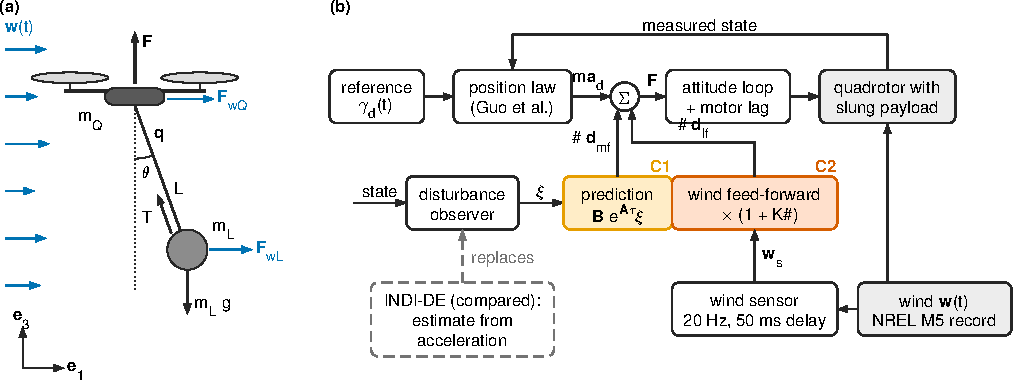
\includegraphics[width=\linewidth]{p2_fig1_system.pdf}
\caption{(a) Plant P2 in side view: quadrotor (mass \(m_Q\)) and payload (\(m_L\)) on a cable of length \(L\) along \(\boldsymbol q\), thrust \(\boldsymbol F\), cable tension \(T\), wind \(\boldsymbol w(t)\) and the wind forces \(\boldsymbol F_{wQ}\) and \(\boldsymbol F_{wL}\) on the two bodies. (b) Controller: the position law of Guo et al., the disturbance observer with the prediction of C1, and the measured-wind feed-forward with the payload-drag factor of C2; in the comparison, INDI-DE replaces the observer's estimate.}\label{fig:1}
\end{figure}


\begin{table}[!htbp]
\caption{Parameters of plant P2 and of the controllers.}\label{tab:param}
\setlength{\tabcolsep}{3pt}
\begin{tabular}{@{}>{\raggedright\arraybackslash}p{0.33\linewidth}>{\raggedright\arraybackslash}p{0.39\linewidth}>{\raggedright\arraybackslash}p{0.2\linewidth}@{}}
\toprule
quantity & value & source \\
\midrule
quadrotor mass $m_Q$ & 1.121 kg & Guo et al. \cite{guo2020} \\
payload mass $m_p$ & 0.5 kg (sensitivity 0.25, 0.65) & this work \\
cable length $L$ & 1 m (sensitivity 0.5, 1.5) & this work \\
cable damping ratio $\zeta_s$ & 0.05 & this work \\
payload drag-area ratio $K = (C_DA)_L/(C_DA)_Q$ & 0.5 & this work \\
wind-force gain $K_w$ & 0.2 N/(m/s) at $U_{ref}$ 5 m/s & derived (Section~\ref{sec:wind-and-the-two-disturbance-paths}) \\
motor lag $\tau_m$ & 17 ms (stress test 25, 30 ms) & this work \\
rotor force limit $f_{\max}$ & 7.668 N & this work \\
total thrust limit & 27.603 N & this work \\
torque limit & 0.5 N m per axis & this work (assumed) \\
tilt clamp & 30\textdegree{} & this work \\
position loop / motion capture & 125 Hz, delay 8 ms, noise SD 0.2 mm & this work \\
attitude loop / IMU & 1000 Hz; noise density acc 0.00177 (m/s$^2$)/$\sqrt{\mathrm{Hz}}$, gyro 0.000122 (rad/s)/$\sqrt{\mathrm{Hz}}$ & this work \\
wind sensor & 20 Hz, delay 50 ms, noise-free & this work \\
$\boldsymbol K_\gamma$ (position) & diag(12, 12, 35) & Guo et al. \cite{guo2020} \\
$\boldsymbol K_v$ (velocity) & diag(8, 8, 18) & Guo et al. \cite{guo2020} \\
$\boldsymbol K_\eta$ / $\boldsymbol K_\omega$ (attitude) & diag(2.16, 1.92, 0.59) / diag(0.2, 0.12, 0.12) & Guo et al. \cite{guo2020} \\
attitude ESO $K_{a1}$ / $K_{a2}$ / $K_{a3}$ & 50 / 833 / 3906 ($\times\boldsymbol I_3$) & Guo et al. \cite{guo2020} \\
payload-prediction horizon $\tau$ & 290 ms circle, 0 hover & measured, development set \\
reference-preview horizon $\tau_{prev}$ & 180 ms & measured, development set \\
PAW-MOBADC feed-forward factor $1+\hat K$ & 1.5 ($\hat K = K = 0.5$) & this work \\
INDI-DE filter cut-off $\omega_f$ & 32 Hz & this work \\
\botrule
\end{tabular}
\end{table}

\subsection{Quadrotor and spherical pendulum}\label{sec:quadrotor-and-spherical-pendulum}

With the cable taut, the quadrotor and the payload obey

\begin{equation}
m_Q\dot{\boldsymbol v}_Q = \boldsymbol F - m_Q g\boldsymbol e_3 + T\boldsymbol q + \boldsymbol F_{wQ} - \boldsymbol F_d
\label{eq:p2-quad}
\end{equation}
\begin{equation}
m_L\ddot{\boldsymbol x}_L = -m_L g\boldsymbol e_3 - T\boldsymbol q + \boldsymbol F_{wL} + \boldsymbol F_d,\qquad \boldsymbol x_L = \boldsymbol x_Q + L\boldsymbol q
\label{eq:p2-load}
\end{equation}
with the cable direction on the sphere

\begin{equation}
\dot{\boldsymbol q} = \boldsymbol\omega\times\boldsymbol q,\qquad \dot{\boldsymbol\omega} = \tfrac{1}{L}\,\boldsymbol q\times\Big[\frac{\boldsymbol F_{wL}+\boldsymbol F_d}{m_L} - \frac{\boldsymbol F + \boldsymbol F_{wQ} - \boldsymbol F_d}{m_Q}\Big]
\label{eq:p2-sphere}
\end{equation}
and the tension that keeps the cable length fixed,

\begin{equation}
T = \mu\Big[\frac{\boldsymbol q\cdot\boldsymbol F_{wL}}{m_L} - \frac{\boldsymbol q\cdot(\boldsymbol F + \boldsymbol F_{wQ})}{m_Q} + L\lVert\dot{\boldsymbol q}\rVert^2\Big],\qquad \mu = \frac{m_Q m_L}{m_Q + m_L}.
\label{eq:p2-tension}
\end{equation}

Without wind and damping these equations reduce to the taut-cable model of Sreenath et al. \cite{sreenath2013}. A cable that goes slack (\(T \le 0\)), where that model becomes hybrid, is flagged and its segment leaves the evaluation. Air drag alone damps small swings too weakly \cite{zhu2025}, so the cable damping is an internal force on both bodies,

\begin{equation}
\boldsymbol F_d = -c\,L\,(\boldsymbol\omega\times\boldsymbol q),\qquad c = 2\zeta_s\omega_n m_L,\qquad \omega_n = \sqrt{g/L},
\label{eq:p2-damp}
\end{equation}
the viscous damping of a linear oscillator written with its damping ratio, here \(\zeta_s = 0.05\). The attitude dynamics are those of Guo et al. \cite{guo2020, raffo2010}, with full Euler-angle inertia and Coriolis terms, and the thrust direction follows the attitude:

\begin{equation}
\boldsymbol M(\boldsymbol\eta)\ddot{\boldsymbol\eta} + \boldsymbol C(\boldsymbol\eta,\dot{\boldsymbol\eta})\dot{\boldsymbol\eta} = \boldsymbol\tau,\qquad \boldsymbol F = f\,\boldsymbol R(\boldsymbol\eta)\boldsymbol e_3.
\label{eq:rot}
\end{equation}
\subsection{Wind and the two disturbance paths}\label{sec:wind-and-the-two-disturbance-paths}

Both bodies feel quadratic drag on their velocity relative to the air,

\begin{equation}
\boldsymbol F_w = \tfrac12\rho\,(C_DA)\,\lVert\boldsymbol w - \boldsymbol v\rVert(\boldsymbol w - \boldsymbol v),
\label{eq:drag}
\end{equation}
with the airframe's drag area chosen so that it feels 1.0 N in a 5 m/s wind and the payload's drag area a fraction \(K\) of it:

\begin{equation}
\tfrac12\rho(C_DA)_Q = K_w/U_{ref},\qquad (C_DA)_L = K\,(C_DA)_Q.
\label{eq:drag-cal}
\end{equation}

In the controller's model \cite{guo2020} the disturbances are the cable force and the wind on the airframe,

\begin{equation}
\boldsymbol d_{mf} = T\boldsymbol q - \boldsymbol F_d,\qquad \boldsymbol d_{lf} = \boldsymbol F_{wQ}.
\label{eq:dist-map}
\end{equation}

The wind on the payload is absent from \(\boldsymbol d_{lf}\): it reaches the vehicle only through the tension, mixed into \(\boldsymbol d_{mf}\) with the inertial and gravitational load force. This is the gap C2 closes.

\subsection{Actuators and sensors}\label{sec:actuators-and-sensors}

Each motor is a first-order lag,

\begin{equation}
\dot f_i = (f_{i,cmd} - f_i)/\tau_m,\qquad \tau_m = 17\ \mathrm{ms},
\label{eq:motor}
\end{equation}
behind the allocation of Guo et al.~with rotor-force and torque saturation:

\begin{equation}
[f;\boldsymbol\tau] = \boldsymbol\Gamma[f_1;\dots;f_4],\qquad f_i = \mathrm{sat}_{[0,f_{\max}]}\big(\boldsymbol\Gamma^{-1}[f;\mathrm{sat}(\boldsymbol\tau)]\big).
\label{eq:alloc}
\end{equation}

The attitude reference inverts the force direction with a 30\textdegree{} tilt clamp and a total-thrust limit. The position loop runs at 125 Hz on motion-capture positions with 8 ms delay, the attitude loop at 1 kHz, and the wind sensor samples at 20 Hz with one sample of delay:

\begin{equation}
\boldsymbol w_s(t_k) = \boldsymbol w(t_k - 0.05\ \mathrm{s}),\qquad \boldsymbol a_{meas} = \boldsymbol a_Q + \boldsymbol n_a.
\label{eq:sensors}
\end{equation}

The accelerometer returns the inertial acceleration plus noise, without the gravity leakage that an attitude error causes in a real specific-force measurement. This choice favours the acceleration-based comparison method; its consequence is quantified with an explicit bias in Section~\ref{sec:measurement-versus-prediction-on-the-circle}.

\section{Controllers}\label{sec:controllers}



\subsection{The baseline and its variants}\label{sec:the-baseline-and-its-variants}

The position law of Guo et al. \cite{guo2020} is

\begin{equation}
\boldsymbol a_d = \boldsymbol K_\gamma\boldsymbol e_\gamma + \boldsymbol K_v\boldsymbol e_v + g\boldsymbol e_3 + \ddot{\boldsymbol\gamma}_d,\qquad \boldsymbol F = m\boldsymbol a_d - \hat{\boldsymbol d}_{mf} - \hat{\boldsymbol d}_{lf},
\label{eq:guo-law}
\end{equation}
with the published gains (Table~\ref{tab:param}). The payload estimate \(\hat{\boldsymbol d}_{mf}\) comes from a disturbance observer whose internal model is the exosystem

\begin{equation}
\dot{\boldsymbol\xi} = \boldsymbol A\boldsymbol\xi,\qquad \boldsymbol d_m = \boldsymbol B\boldsymbol\xi,\qquad \boldsymbol A_i = \begin{bmatrix}0&\sigma_i\\-\sigma_i&0\end{bmatrix},
\label{eq:exo}
\end{equation}
with \(\sigma\) the angular rate of the planned trajectory, and \(\hat{\boldsymbol d}_{lf}\) from a position extended state observer. The controllers compared are:


\begin{center}\footnotesize
\begin{tabular}{@{}p{0.32\linewidth}p{0.6\linewidth}@{}}
\toprule
\textbf{name} & \textbf{definition} \\
\midrule
\textbf{PID} & Guo's laws with every estimate switched off \\
\textbf{DO}, \textbf{ESO} & Guo's controller with only the disturbance observer, or only the two extended state observers \\
\textbf{MOBADC} & Guo's controller as published \cite{guo2020} \\
\textbf{MOBADC-DC} & MOBADC with a constant (DC) mode added to the observer's internal model \\
\textbf{MOBADC-W} & MOBADC-DC with the measured-wind feed-forward in place of the position observer (Section~\ref{sec:measured-wind-feed-forward}) \\
\textbf{MOBADC-W + preview} & MOBADC-W with the reference acceleration taken \(\tau_{prev}\) ahead \\
\textbf{PA-MOBADC} & MOBADC-W with the payload estimate predicted \(\tau\) ahead (C1) \\
\textbf{PAW-MOBADC} & PA-MOBADC with the payload's drag in the wind feed-forward (C2) - the proposed method \\
\textbf{INDI-DE} & INDI-type acceleration-based disturbance estimation (Section~\ref{sec:comparison-methods}) \\
\botrule
\end{tabular}
\end{center}


PID and DO are also run with the known payload weight added to their force command (``+ trim''). The DC mode lets the observer hold the static part of the cable force, which a purely harmonic model cannot represent.

\subsection{Measured-wind feed-forward}\label{sec:measured-wind-feed-forward}

MOBADC-W replaces the position extended state observer by the controller's drag model fed with the measured wind,

\begin{equation}
\hat{\boldsymbol d}_{lf} = \frac{K_w}{U_{ref}}\lVert\boldsymbol w_s - \boldsymbol v_Q\rVert(\boldsymbol w_s - \boldsymbol v_Q).
\label{eq:wind-ff}
\end{equation}

A measured disturbance needs no estimator and therefore no estimator bandwidth \cite{chen2016}; MOBADC-W is the reference against which both contributions are measured, because it isolates what the wind measurement alone achieves.

\subsection{C1 - compensation of the loop delay (PA-MOBADC)}\label{sec:c1-compensation-of-the-loop-delay-pa-mobadc}

\textbf{Why the delay matters.} The force command computed at time \(t\) acts on the vehicle after a closed-loop delay \(\tau_d\) (sampling, motor lag, attitude response). Without prediction the compensation error at the moment the command acts is

\begin{equation}
\boldsymbol e_{mf}(t) = \boldsymbol d_{mf}(t+\tau_d) - \boldsymbol B\hat{\boldsymbol\xi}(t) = \boldsymbol B\tilde{\boldsymbol\xi}(t) + \big[\boldsymbol d_{mf}(t+\tau_d) - \boldsymbol d_{mf}(t)\big],\qquad \tilde{\boldsymbol\xi} = \boldsymbol\xi - \hat{\boldsymbol\xi}.
\label{eq:lag-err}
\end{equation}

The bracket does not vanish when the observer is exact. For one harmonic of amplitude \(a\) and frequency \(\sigma\) its magnitude is \(2a\,|\sin(\sigma\tau_d/2)|\); on the circle of this study (\(\sigma = 1.575\) rad/s) and with the delay measured below (\(\tau_d = 290\) ms) this is 0.45 of the amplitude (Fig.~\ref{fig:2}a). A perfect estimate applied late leaves almost half of the periodic payload force uncancelled, and a faster estimator cannot change that.


\begin{figure}[!htbp]
\centering
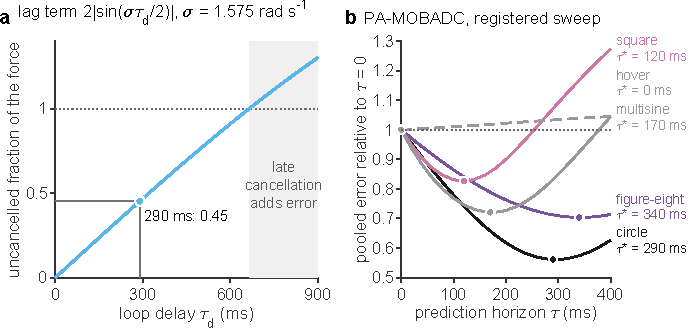
\includegraphics[width=\linewidth]{ijdc_horizon.pdf}
\caption{Why the loop delay matters. (a) Fraction of a harmonic payload force of frequency \(\sigma\) that a cancellation late by the loop delay \(\tau_d\) leaves uncancelled, \(2|\sin(\sigma\tau_d/2)|\), at the frequency of the circle; in the shaded range a late cancellation adds error. (b) Pooled error of PA-MOBADC against the prediction horizon \(\tau\) in the registered sweeps on the development segments, relative to its value at \(\tau = 0\); dots: the chosen horizon \(\tau^*\).}\label{fig:2}
\end{figure}


\textbf{Prediction through the exosystem.} The observer's internal model is the generator of the disturbance, so the estimate can be carried over the delay with it:

\begin{equation}
\hat{\boldsymbol d}_{mf}(t+\tau) = \boldsymbol B\,e^{\boldsymbol A\tau}\hat{\boldsymbol\xi}(t).
\label{eq:pred}
\end{equation}

Each \(2\times2\) block of \(e^{\boldsymbol A\tau}\) is a rotation, so the prediction costs two trigonometric evaluations per mode, and the DC mode is unchanged. For a harmonic mode this is the shift of Bobtsov and Pyrkin \cite{bobtsov2012} with unit gain and no plant phase, because the payload force enters the force channel directly.

\begin{proposition}[prediction does not amplify the estimation error]
Let \(\boldsymbol A\) be block diagonal with zero and skew-symmetric \(2\times2\) blocks. With \(\tau = \tau_d\) the compensation error of \eqref{eq:pred} is

\begin{equation}
\boldsymbol e_{mf}(t) = \boldsymbol B\,e^{\boldsymbol A\tau}\tilde{\boldsymbol\xi}(t) + \big[\boldsymbol d_{mf}(t+\tau) - \boldsymbol B\,e^{\boldsymbol A\tau}\boldsymbol\xi(t)\big],\qquad \lVert\boldsymbol B\,e^{\boldsymbol A\tau}\tilde{\boldsymbol\xi}(t)\rVert \le \lVert\boldsymbol B\rVert\,\lVert\tilde{\boldsymbol\xi}(t)\rVert .
\label{eq:pred-err}
\end{equation}
\end{proposition}
\begin{proof}
\(e^{\boldsymbol A\tau}\) is block diagonal with identity and rotation blocks, hence orthogonal, so \(\lVert e^{\boldsymbol A\tau}\boldsymbol x\rVert = \lVert\boldsymbol x\rVert\) for every \(\boldsymbol x\) and every \(\tau\); the bound follows from \(\lVert\boldsymbol B\boldsymbol y\rVert \le \lVert\boldsymbol B\rVert\lVert\boldsymbol
y\rVert\).
\end{proof}

The estimation part of the error is therefore no larger than without prediction, for any horizon, while the bracket - the deviation of the true force from the exosystem over the horizon - is zero for a force that follows the internal model and replaces the lag term of \eqref{eq:lag-err} otherwise. Prediction trades a phase error that is certain for a model error that is small when the internal model is right. The horizon was measured on the development set by a registered sweep (Section~\ref{sec:c1-compensation-of-the-loop-delay}): \(\tau = 290\) ms on the circle; in hover, where the payload force has no orbital frequency, the minimum lies at \(\tau = 0\).

\subsection{C2 - payload drag in the wind feed-forward (PAW-MOBADC, the proposed method)}\label{sec:c2-payload-drag-in-the-wind-feed-forward-paw-mobadc-the-proposed-method}

The feed-forward of Section~\ref{sec:measured-wind-feed-forward} accounts for the wind on the airframe only. Adding \eqref{eq:p2-quad} and \eqref{eq:p2-load} removes the tension and the cable damping, which are internal forces of the two-body system:

\begin{equation}
m_Q\dot{\boldsymbol v}_Q + m_L\ddot{\boldsymbol x}_L = \boldsymbol F - (m_Q+m_L)g\boldsymbol e_3 + \boldsymbol F_{wQ} + \boldsymbol F_{wL}.
\label{eq:balance}
\end{equation}

The thrust must therefore balance the wind force on both bodies. The payload's drag area is \(K\) times the airframe's \eqref{eq:drag-cal}; when the payload meets the same wind with the velocity of the vehicle, \eqref{eq:drag} gives \(\boldsymbol F_{wL} = K\boldsymbol F_{wQ}\), and the wind force the thrust has to balance is \((1+K)\boldsymbol F_{wQ}\). The controller uses its assumed ratio \(\hat K\) and scales the measured-wind term:

\begin{equation}
\hat{\boldsymbol d}_{lf} = (1+\hat K)\,\frac{K_w}{U_{ref}}\lVert\boldsymbol w_s - \boldsymbol v_Q\rVert(\boldsymbol w_s - \boldsymbol v_Q),\qquad \hat K = 0.5.
\label{eq:paw-ff}
\end{equation}
\begin{proposition}[residual of the static term]
With \(\boldsymbol r_Q = \boldsymbol w - \boldsymbol v_Q\), \(\boldsymbol r_L = \boldsymbol w - \boldsymbol v_L\) and \(k = K_w/U_{ref}\), the part of the payload's wind force that \eqref{eq:paw-ff} leaves uncompensated, measurement delay apart, is

\begin{equation}
\begin{gathered}
\boldsymbol F_{wL} - \hat K k\lVert\boldsymbol r_Q\rVert\boldsymbol r_Q = (K-\hat K)\,k\lVert\boldsymbol r_Q\rVert\boldsymbol r_Q + K k\big(\lVert\boldsymbol r_L\rVert\boldsymbol r_L - \lVert\boldsymbol r_Q\rVert\boldsymbol r_Q\big),\\ \big\lVert\lVert\boldsymbol r_L\rVert\boldsymbol r_L - \lVert\boldsymbol r_Q\rVert\boldsymbol r_Q\big\rVert \le \big(\lVert\boldsymbol r_L\rVert + \lVert\boldsymbol r_Q\rVert\big)\,L\lVert\boldsymbol\omega\rVert .
\end{gathered}
\label{eq:ff-err}
\end{equation}
\end{proposition}
\begin{proof}
The decomposition is algebraic. For the bound, \(\lVert\boldsymbol a\rVert\boldsymbol a - \lVert\boldsymbol
b\rVert\boldsymbol b = \lVert\boldsymbol a\rVert(\boldsymbol a - \boldsymbol b) + (\lVert\boldsymbol a\rVert -
\lVert\boldsymbol b\rVert)\boldsymbol b\), whose norm is at most \((\lVert\boldsymbol a\rVert + \lVert\boldsymbol
b\rVert)\lVert\boldsymbol a - \boldsymbol b\rVert\), and \(\boldsymbol r_Q - \boldsymbol r_L = \boldsymbol v_L -
\boldsymbol v_Q = L\,\boldsymbol\omega\times\boldsymbol q\) has norm at most \(L\lVert\boldsymbol\omega\rVert\).
\end{proof}

The residual has two sources: a wrong assumed ratio, which is proportional to the feed-forward itself, and the relative motion of the load, which is proportional to the swing rate. The static term is exact for a load that moves with the vehicle and degrades gracefully with swing; Section~\ref{sec:c2-payload-drag-in-the-wind-feed-forward} measures both sources by varying \(\hat K\) and by flying trajectories with different swing.

\subsection{Boundedness of the closed loop}\label{sec:boundedness-of-the-closed-loop}

Both additions change only the compensation signal \(\hat{\boldsymbol d}_{mf} + \hat{\boldsymbol d}_{lf}\) in \eqref{eq:guo-law}; the feedback laws, the observers and their gains are those of Guo et al.\@ Let \(\boldsymbol e_d\) be the total compensation error at the moment the command acts. If the translational and attitude loops of the baseline are input-to-state stable with respect to \(\boldsymbol e_d\), with gain \(\gamma\), the tracking error of every controller in Section~\ref{sec:the-baseline-and-its-variants} is ultimately bounded by \(\gamma(\sup_t\lVert\boldsymbol e_d(t)\rVert)\), and the question reduces to the size of \(\boldsymbol e_d\):

\begin{equation}
\lVert\boldsymbol e_d\rVert \le \lVert\boldsymbol B\rVert\,\lVert\tilde{\boldsymbol\xi}\rVert + \lVert\boldsymbol d_{mf}(t+\tau) - \boldsymbol B e^{\boldsymbol A\tau}\boldsymbol\xi(t)\rVert + \lVert\boldsymbol F_{wQ}(t+\tau_d) - \hat{\boldsymbol d}_{lf}(t)\rVert .
\label{eq:ed-bound}
\end{equation}

The first term is bounded because the observer's error dynamics are stable and driven by the bounded mismatch between the payload force and the exosystem \cite{chen2004}, and Proposition 1 shows that prediction does not enlarge it; the second because the payload force and the exosystem output are bounded on bounded trajectories. The third contains, by design, the excess \(\hat K k\lVert\boldsymbol r_Q\rVert\boldsymbol r_Q\) that offsets the load's wind force carried by \(\boldsymbol d_{mf}\) through the tension; it is bounded because the wind and the velocities are bounded, and Proposition 2 bounds what the offset leaves. Neither addition can therefore destabilise a loop that is input-to-state stable with respect to its compensation error; both move the ultimate bound, which is what Section~\ref{sec:results} measures. The assumption concerns the baseline alone: it is the property on which composite disturbance-observer controllers rest \cite{chen2004}; for this baseline its authors prove a bounded error of the position loop and asymptotic stability of the attitude loop under a small-angle linearisation \cite{guo2020}. Section~\ref{sec:the-boundedness-assumption-and-the-published-gains} shows that the assumption fails for the published gains at motor lags of 25 ms and above, independently of either addition.

\subsection{Comparison methods}\label{sec:comparison-methods}

\textbf{INDI-DE} estimates the total disturbance from the measured acceleration, as the outer loop of incremental nonlinear dynamic inversion \cite{smeur2018}:

\begin{equation}
\hat{\boldsymbol d}_{mf} = H(z)\big[m\boldsymbol a_{meas} - \hat{\boldsymbol F}_{thr} + mg\boldsymbol e_3\big],\qquad \hat{\boldsymbol d}_{lf} = 0,
\label{eq:h3}
\end{equation}
with \(H\) a second-order low-pass filter whose cut-off, 32 Hz, is the best value of a registered sweep and therefore chosen in favour of the competitor, and the thrust estimated through the nominal motor lag. Guo's attitude loop is kept; there is no inner INDI loop. \textbf{MBP} (model-based payload predictor) replaces the static term of C2 by an open-loop pendulum prediction of the payload force. \textbf{The oracle} of C3 feeds the wind channel with the true future wind,

\begin{equation}
\hat{\boldsymbol d}_{lf} = \frac{K_w}{U_{ref}}\lVert\boldsymbol w(t+\tau_w) - \boldsymbol v_Q\rVert(\boldsymbol w(t+\tau_w) - \boldsymbol v_Q),
\label{eq:oracle}
\end{equation}
an upper bound on what any wind predictor could add through the controller's force model.

\section{Experimental design}\label{sec:experimental-design}



\subsection{Wind data and segments}\label{sec:wind-data-and-segments}

Measured wind comes from the sonic anemometers of the M5 tower at the National Wind Technology Center of NREL, at heights of 61 and 74 m, sampled at 20 Hz. Each run lasts 200 s; statistics use \(t \ge 140\) s. A segment enters a trajectory's set only if the vehicle can hold the trajectory against the static wind force at the segment's mean wind speed with tilt and thrust within 80 \% of their limits; on the circle (radius 0.8 m, angular rate 1.575 rad/s) this admits mean winds up to 8.02 m/s (Fig.~\ref{fig:3}).


\begin{figure}[!htbp]
\centering
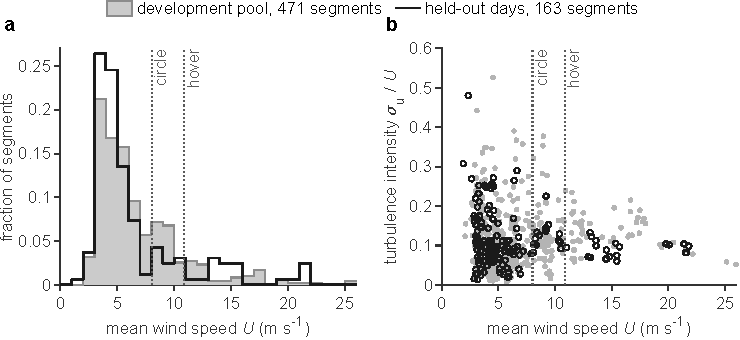
\includegraphics[width=\linewidth]{ijdc_wind.pdf}
\caption{Measured wind of the development pool and of the held-out days: (a) distribution of the mean wind speed \(U\) per segment, (b) turbulence intensity against \(U\). Dotted: the largest mean wind at which the vehicle can hold the circle and the hover point (Section~\ref{sec:wind-data-and-segments}).}\label{fig:3}
\end{figure}


\begin{itemize}
\tightlist
\item
  \textbf{Development pool:} 471 segments from 46 days. Every horizon, every post-hoc finding and every development-set number comes from it. The main circle set holds 134 segments (42 days, at most four per day), the hover set 139 segments (43 days); sensitivity tables use one segment per day (40 on the circle, 43 in hover).
\item
  \textbf{Held-out set:} 14 days chosen by a hash rule before download and opened once, after every claim, threshold and runner had been frozen. Two further days of the manifest had been inspected segment by segment while the wind pipeline was built and were excluded before any controller run; the remaining days had contributed only to pooled wind statistics of that earlier stage \cite{nosek2018}.
\end{itemize}

\subsection{Metric and statistics}\label{sec:metric-and-statistics}

The metric of a segment is the mean position-error norm over the window,

\begin{equation}
m_i = \operatorname{mean}_{t\ge140}\lVert\boldsymbol\gamma_d - \boldsymbol\gamma\rVert,
\label{eq:metric}
\end{equation}
pooled over a set as

\begin{equation}
P = \sqrt{\operatorname{mean}_i m_i^2},\qquad \Delta = P_a/P_b - 1,\qquad h = 1 - P_b/P_a.
\label{eq:pool}
\end{equation}

Because segments of one day share weather, every ratio carries a paired delete-one-day jackknife standard error,

\begin{equation}
\mathrm{SE} = \sqrt{\tfrac{D-1}{D}\textstyle\sum_{d=1}^{D}(\hat\theta_{(-d)} - \bar\theta)^2},
\label{eq:jack}
\end{equation}
with \(D\) the number of days, beside the range of leave-one-segment-out values and the median of the per-day values. One table is scored on one set of segments: a segment on which any column fails leaves that table. The control effort is reported as the RMS oscillation of the commanded rotor forces about their own means, and the payload swing as the RMS cable angle.

\subsection{Registration and held-out confirmation}\label{sec:registration-and-held-out-confirmation}

Each claim was written, with its test and threshold, in a dated register before its data were opened; a finding made after seeing development data was labelled post hoc and could only become a claim by being registered and tested on the held-out days \cite{nosek2018, munafo2017}. The held-out claims are:

\begin{itemize}
\tightlist
\item
  \textbf{D2} (C1): \(\Delta\) = PA-MOBADC / MOBADC-W \textminus{} 1 on the circle; confirmed if \(\Delta \le -15\) \% and \(\Delta\) + 1.65 SE \textless{} 0.
\item
  \textbf{H-static} and \textbf{H-static-circle} (C2): \(h\) = 1 \textminus{} PAW-MOBADC / PA-MOBADC, in hover and on the circle, scored on the segments where PA-MOBADC is not at its tilt clamp; confirmed if the per-day median is at least 10 \%, \(h\) \textminus{} 1.65 SE \textgreater{} 0, and PAW-MOBADC fails on at most one segment where PA-MOBADC runs.
\item
  \textbf{H-hover} (C3, one post-hoc group): \(h\) = 1 \textminus{} oracle / PA-MOBADC in strong hover wind relative to the envelope.
\end{itemize}

Every registered test with a pass/fail outcome is reported as it stands. 2 of the 7 registered predictions scored in this paper were missed: the C3 headroom gate (no group had headroom) and the acceptance of MBP.


\begin{center}\footnotesize
\begin{tabular}{@{}p{0.46\linewidth}p{0.22\linewidth}p{0.22\linewidth}@{}}
\toprule
\textbf{where} & \textbf{scored} & \textbf{missed} \\
\midrule
development gates: D2 gate, C3 headroom gate, MBP acceptance, eligibility of PAW-MOBADC for the held-out test & 4 & 2 \\
held-out claims: D2, H-static, H-static-circle (H-hover not scorable: one segment) & 3 & 0 \\
\botrule
\end{tabular}
\end{center}


\subsection{Reproduction}\label{sec:reproduction}

The development-set results were computed twice. After the original runs, the complete pipeline - download of the public wind records, export of the segments, measurement of every horizon and every simulation - was executed again, independently, on a different operating system. All 39 development-set statistics of Section~\ref{sec:results} agree to the printed digit between the two executions, and the additional checks of Section~\ref{sec:c2-payload-drag-in-the-wind-feed-forward} come from the second one.

\subsection{Use of AI-assisted tools}\label{sec:use-of-ai-assisted-tools}

AI-assisted tools were used to help write the simulation and analysis code and to edit the manuscript. The design of the study, the registered claims, the analyses and the conclusions are the authors', who checked every result and take full responsibility for the content.

\section{Results}\label{sec:results}



\subsection{Main comparison}\label{sec:main-comparison}

\textbf{The proposed PAW-MOBADC lowers the pooled error of MOBADC on the circle from 0.0451 m to 0.0120 m, by 73.42 \% (SE 6.34), on the development set (133 segments on 42 days), and from 0.0405 m to 0.00873 m, by 78.44 \% (SE 0.61), on the 56 held-out segments.} Each of the two additions removes a distinct part of this error (Fig.~\ref{fig:4}, Table~\ref{tab:ablation}). On the held-out circle the measured-wind feed-forward leaves MOBADC-W at 0.0343 m, the delay compensation brings the error to 0.0143 m and the payload-drag term to 0.00873 m; against MOBADC-W, the stronger reference because it already uses the wind measurement, the complete controller lowers the error by 74.57 \% (SE 1.83). In hover the registered horizon is \(\tau = 0\), so PA-MOBADC equals MOBADC-W, and the payload-drag term lowers the error from 0.00680 m to 0.00252 m on the held-out segments where PA-MOBADC is below its tilt clamp. These comparisons are descriptive; the registered claims behind the two steps are those of Sections~\ref{sec:c1-compensation-of-the-loop-delay} and \ref{sec:c2-payload-drag-in-the-wind-feed-forward}. Among the controllers of Guo et al., MOBADC keeps the lowest error on the development circle (Table~\ref{tab:main}), as in their indoor test \cite{guo2020}.


\begin{figure}[!htbp]
\centering
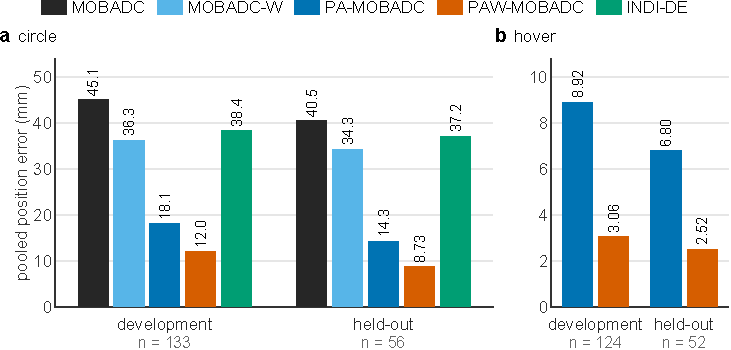
\includegraphics[width=\linewidth]{ijdc_compare.pdf}
\caption{Pooled position error of each controller on the development set and on the held-out days: (a) circle; (b) hover, on the segments where PA-MOBADC is below its tilt clamp (the registered scoring set; with \(\tau = 0\) PA-MOBADC equals MOBADC-W). \(n\): segments.}\label{fig:4}
\end{figure}


\begin{sidewaystable}
\caption{Ablation MOBADC-W $\rightarrow$ PA-MOBADC (C1) $\rightarrow$ PAW-MOBADC (C2): pooled error of each stage on the block's common set of segments and the step changes (SE; leave-one-out range; by-day median). ``unsat.'' = segments on which PA-MOBADC is below its tilt clamp. MOBADC-W was not run in hover.}\label{tab:ablation}
\setlength{\tabcolsep}{3pt}
\begin{tabular}{@{}>{\raggedright\arraybackslash}p{0.14\linewidth}>{\raggedright\arraybackslash}p{0.07\linewidth}>{\raggedright\arraybackslash}p{0.075\linewidth}>{\raggedright\arraybackslash}p{0.075\linewidth}>{\raggedright\arraybackslash}p{0.075\linewidth}>{\raggedright\arraybackslash}p{0.155\linewidth}>{\raggedright\arraybackslash}p{0.155\linewidth}>{\raggedright\arraybackslash}p{0.155\linewidth}@{}}
\toprule
block & segments (days) & MOBADC-W [m] & PA-MOBADC [m] & PAW-MOBADC [m] & C1: PA-MOBADC / MOBADC-W $-$ 1 & C2: PAW-MOBADC / PA-MOBADC $-$ 1 & total: PAW-MOBADC / MOBADC-W $-$ 1 \\
\midrule
circle, development & 133 (42) & 0.03631 & 0.01806 & 0.01199 & $-$50.25 \% (8.31; [$-$57.29, $-$50.14]; $-$62.23) & $-$33.64 \% (8.23; [$-$42.93, $-$32.99]; $-$36.76) & $-$66.99 \% (8.83; [$-$75.63, $-$66.88]; $-$76.61) \\
circle, held-out & 56 (14) & 0.03434 & 0.01432 & 0.00873 & $-$58.30 \% (4.57; [$-$60.66, $-$58.12]; $-$63.88) & $-$39.00 \% (2.91; [$-$39.21, $-$37.59]; $-$35.07) & $-$74.57 \% (1.83; [$-$76.09, $-$74.51]; $-$76.42) \\
hover, development & 137 (43) & -- & 0.02461 & 0.01962 & -- & $-$20.27 \% (42.39; [$-$63.56, $-$19.75]; $-$62.92) & -- \\
hover, development, PA-MOBADC unsat. & 124 (41) & -- & 0.00892 & 0.00306 & -- & $-$65.68 \% (1.59; [$-$65.95, $-$64.50]; $-$62.92) & -- \\
hover, held-out & 56 (14) & -- & 0.01057 & 0.00385 & -- & $-$63.55 \% (1.75; [$-$65.74, $-$62.49]; $-$61.30) & -- \\
\botrule
\end{tabular}
\end{sidewaystable}


\begin{table}[!htbp]
\caption{Eight controllers on the development circle (133 segments, 42 days; one segment left out because PAW-MOBADC stopped on it). Mean = pooled mean position-error norm with day-jackknife SE and by-day median; STD = within-segment standard deviation of the error norm, pooled; $\theta$ RMS = payload cable angle, mostly the steady cone angle on the circle (15.0\textdegree{} without wind). ``+ trim'' = known payload weight added to the force command.}\label{tab:main}
\setlength{\tabcolsep}{3pt}
\begin{tabular}{@{}>{\raggedright\arraybackslash}p{0.19\linewidth}>{\raggedright\arraybackslash}p{0.26\linewidth}>{\raggedright\arraybackslash}p{0.12\linewidth}>{\raggedright\arraybackslash}p{0.1\linewidth}>{\raggedright\arraybackslash}p{0.12\linewidth}>{\raggedright\arraybackslash}p{0.09\linewidth}@{}}
\toprule
controller & mean [m] (SE; by-day median) & median of segment means [m] & STD [m] & median of segment STDs [m] & $\theta$ RMS [\textdegree] \\
\midrule
PID & 0.20100 (0.00645; 0.19624) & 0.17978 & 0.05037 & 0.03050 & 17.29 \\
PID + trim & 0.15348 (0.00827; 0.14731) & 0.12477 & 0.06129 & 0.04630 & 17.29 \\
DO & 0.18416 (0.00656; 0.17930) & 0.16269 & 0.04085 & 0.01503 & 17.08 \\
DO + trim & 0.13956 (0.00847; 0.13295) & 0.11099 & 0.04644 & 0.02361 & 17.08 \\
ESO & 0.07577 (0.00276; 0.07131) & 0.07024 & 0.03608 & 0.01699 & 17.36 \\
MOBADC & 0.04510 (0.00466; 0.03646) & 0.03578 & 0.03321 & 0.01143 & 17.08 \\
INDI-DE & 0.03838 (0.00152; 0.03688) & 0.03685 & 0.02762 & 0.00436 & 17.29 \\
PAW-MOBADC (proposed) & 0.01199 (0.00374; 0.00777) & 0.00764 & 0.02631 & 0.00335 & 16.70 \\
\botrule
\end{tabular}
\end{table}


\textbf{What each step removes.} Fig.~\ref{fig:5} shows the tracking error on one circle and one hover segment, each chosen by a registered rule. On the circle, MOBADC-W flies behind and outside the reference by a nearly constant amount: in the frame of the path its error is an offset along the track and outwards. This is the lag term of \eqref{eq:lag-err}. The payload force turns with the vehicle, so a cancellation that is one loop delay late leaves an error that is constant in the frame of the path. PA-MOBADC removes the offset; what remains follows the wind and is largest in the gusts, and PAW-MOBADC removes most of it. In hover the payload force has no orbital frequency, the error of PA-MOBADC follows the wind directly, and PAW-MOBADC reduces it.


\begin{figure}[!htbp]
\centering
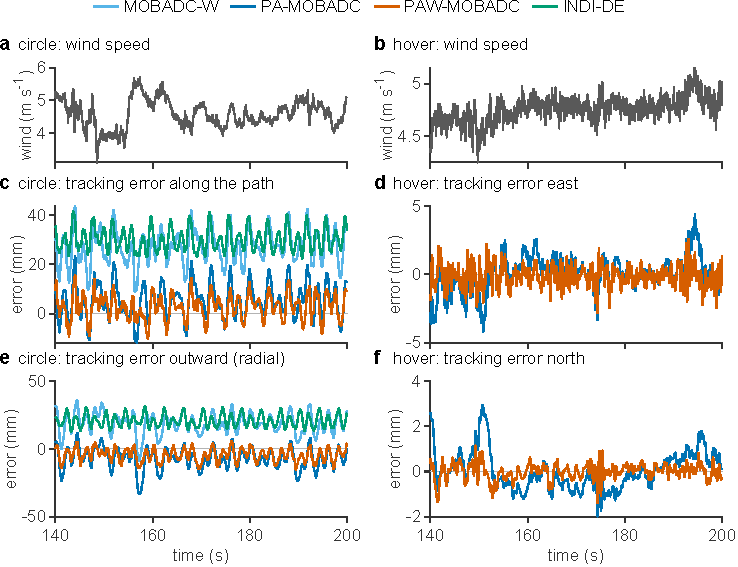
\includegraphics[width=\linewidth]{ijdc_response.pdf}
\caption{Time responses on one development circle segment (left) and one development hover segment (right), each chosen by a registered rule: (a, b) horizontal wind speed; (c, e) tracking error of the vehicle along the path and outward from the centre of the circle; (d, f) tracking error east and north.}\label{fig:5}
\end{figure}


\textbf{Across segments} the same division holds (Fig.~\ref{fig:6}). On the development circle the error of MOBADC-W hardly depends on the mean wind speed - it is set by the delay, not by the wind - whereas the error of PA-MOBADC grows with the wind speed and that of PAW-MOBADC stays nearly flat. In hover the error of both grows with the wind, and PAW-MOBADC stays below PA-MOBADC in every wind-speed bin.



\begin{figure}[!htbp]
\centering
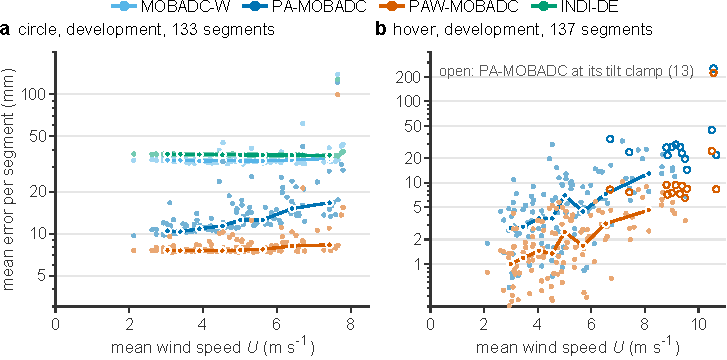
\includegraphics[width=\linewidth]{ijdc_windspeed.pdf}
\caption{Mean position error per segment against the mean wind speed of the segment, development sets: (a) circle, (b) hover. Dots: segments; lines: medians of eight bins with equal numbers of segments; open circles in (b): segments on which PA-MOBADC reaches its tilt clamp.}\label{fig:6}
\end{figure}

\subsection{C1 - compensation of the loop delay}\label{sec:c1-compensation-of-the-loop-delay}

The registered development gate D2 passed: PA-MOBADC lowered the pooled error of MOBADC-W by 50.33 \% (SE 8.28, by-day median \textminus{}62.23 \%), from 0.0363 m to 0.0180 m. \textbf{On the held-out days D2 was confirmed: \textminus{}58.30 \% (SE 4.57, leave-one-out range {[}\textminus{}60.66, \textminus{}58.12{]}, by-day median \textminus{}63.88 \%), from 0.0343 m to 0.0143 m} (Table~\ref{tab:claims}). The size of the gain agrees with the argument of Section~\ref{sec:c1-compensation-of-the-loop-delay-pa-mobadc}: a 290 ms delay leaves 0.45 of a harmonic payload force uncancelled (Fig.~\ref{fig:2}a), and prediction removes most of it. The horizon comes from the registered sweep of Fig.~\ref{fig:2}b: on the circle the pooled error has its minimum at 290 ms, and in hover, where the payload force has no orbital frequency, at the lower edge of the grid, \(\tau = 0\).

\begin{sidewaystable}
\caption{The claims on the development set and on the held-out days (Section~\ref{sec:registration-and-held-out-confirmation}): value, day-jackknife SE, leave-one-segment-out range, by-day median, and the verdict of the registered test. ``unsat.'' = scored on the segments on which PA-MOBADC is below its tilt clamp; ``1/day'' = one segment per day.}\label{tab:claims}
\setlength{\tabcolsep}{3pt}
\begin{tabular}{@{}>{\raggedright\arraybackslash}p{0.21\linewidth}>{\raggedright\arraybackslash}p{0.13\linewidth}>{\raggedright\arraybackslash}p{0.09\linewidth}>{\raggedright\arraybackslash}p{0.07\linewidth}>{\raggedright\arraybackslash}p{0.05\linewidth}>{\raggedright\arraybackslash}p{0.12\linewidth}>{\raggedright\arraybackslash}p{0.07\linewidth}>{\raggedright\arraybackslash}p{0.07\linewidth}>{\raggedright\arraybackslash}p{0.08\linewidth}@{}}
\toprule
claim & set & role & value & SE & leave-one-out range & by-day median & segments (days) & verdict \\
\midrule
D2: PA-MOBADC / MOBADC-W $-$ 1 & dev., circle & registered gate & $-$50.33 \% & 8.28 & [$-$57.35, $-$50.22] & $-$62.23 \% & 134 (42) & passed \\
D2: PA-MOBADC / MOBADC-W $-$ 1 & held-out, circle & registered claim & $-$58.30 \% & 4.57 & [$-$60.66, $-$58.12] & $-$63.88 \% & 56 (14) & confirmed \\
H-static: 1 $-$ PAW-MOBADC / PA-MOBADC (unsat.) & dev., hover & post hoc & +65.68 \% & 1.59 & [+64.50, +65.95] & +62.92 \% & 124 (41) & -- \\
H-static, all segments & dev., hover & post hoc & +20.27 \% & 42.39 & [+19.75, +63.56] & +62.92 \% & 137 (43) & -- \\
H-static: 1 $-$ PAW-MOBADC / PA-MOBADC (unsat.) & held-out, hover & registered claim & +63.00 \% & 1.37 & [+61.12, +64.09] & +61.30 \% & 52 (14) & confirmed \\
H-static-circle: 1 $-$ PAW-MOBADC / PA-MOBADC & dev., circle, 1/day & post hoc & +43.67 \% & 2.16 & [+42.33, +43.92] & +34.59 \% & 39 (39) & -- \\
H-static-circle (unsat.) & held-out, circle & registered claim & +37.18 \% & 3.04 & [+36.19, +37.40] & +35.07 \% & 53 (14) & confirmed \\
H-hover: 1 $-$ oracle / PA-MOBADC (unsat.) & dev., hover, strong wind & post hoc & +41.52 \% & 0.15 & [+41.44, +41.63] & +41.47 \% & 10 (5) & -- \\
H-hover: 1 $-$ oracle / PA-MOBADC (unsat.) & held-out, hover, strong wind & registered claim & +41.92 \% & -- & [+41.92, +41.92] & +41.92 \% & 1 (1) & not scorable \\
\botrule
\end{tabular}
\end{sidewaystable}


The gain holds on the other planned trajectories, \textminus{}45.41 \% on the figure-eight and \textminus{}24.80 \% on the square, and across every payload mass, cable length and their combinations, between \textminus{}58.9 \% and \textminus{}34.9 \% (Table~\ref{tab:sens}). It is smallest where the payload is light and the cable long, that is, where the periodic payload force is smallest relative to the wind. The reference preview (MOBADC-W + preview) compensates the same delay along the planned trajectory and gives a comparable gain, \textminus{}62.40 \% on the held-out days; Section~\ref{sec:two-realisations-of-delay-compensation} compares the two realisations.


\begin{sidewaystable}
\caption{C1 across payload mass $m_p$ [kg] and cable length $L$ [m] on the development circle, one segment per day: horizon, segments used, pooled errors and the changes against MOBADC-W (SE; leave-one-out range; by-day median). The light-payload rows are pooled on the segments inside their wind envelope $U \le U_{\max}$.}\label{tab:sens}
\setlength{\tabcolsep}{3pt}
\begin{tabular}{@{}>{\raggedright\arraybackslash}p{0.09\linewidth}>{\raggedright\arraybackslash}p{0.05\linewidth}>{\raggedright\arraybackslash}p{0.1\linewidth}>{\raggedright\arraybackslash}p{0.07\linewidth}>{\raggedright\arraybackslash}p{0.07\linewidth}>{\raggedright\arraybackslash}p{0.07\linewidth}>{\raggedright\arraybackslash}p{0.07\linewidth}>{\raggedright\arraybackslash}p{0.18\linewidth}>{\raggedright\arraybackslash}p{0.18\linewidth}@{}}
\toprule
($m_p$, $L$) & $\tau$ [ms] & segments & MOBADC [m] & MOBADC-W [m] & PA-MOBADC [m] & MOBADC-W + preview [m] & PA-MOBADC / MOBADC-W $-$ 1 & (MOBADC-W + preview) / MOBADC-W $-$ 1 \\
\midrule
(0.5, 1.0) nominal & 290 & 40/40 & 0.04369 & 0.03494 & 0.01530 & 0.01355 & $-$56.22 \% (3.23; [$-$58.96, $-$55.94]; $-$64.87) & $-$61.21 \% (3.20; [$-$63.88, $-$60.96]; $-$69.04) \\
(0.25, 1.0) & 290 & 37/40 (2 above $U_{\max}$) & 0.03662 & 0.02935 & 0.01787 & 0.01450 & $-$39.09 \% (1.64; [$-$40.03, $-$38.87]; $-$43.24) & $-$50.58 \% (1.99; [$-$51.63, $-$50.36]; $-$55.96) \\
(0.65, 1.0) & 290 & 40/40 & 0.04604 & 0.03785 & 0.01713 & 0.01322 & $-$54.75 \% (2.32; [$-$56.60, $-$54.51]; $-$61.19) & $-$65.06 \% (3.45; [$-$68.02, $-$64.80]; $-$72.89) \\
(0.5, 0.5) & 330 & 40/40 & 0.04265 & 0.03361 & 0.01380 & 0.01340 & $-$58.95 \% (3.72; [$-$62.15, $-$58.66]; $-$68.86) & $-$60.14 \% (3.06; [$-$62.68, $-$59.90]; $-$67.77) \\
(0.5, 1.5) & 260 & 40/40 & 0.04492 & 0.03642 & 0.01703 & 0.01355 & $-$53.25 \% (2.78; [$-$55.55, $-$52.99]; $-$60.92) & $-$62.80 \% (3.75; [$-$66.04, $-$62.52]; $-$71.85) \\
(0.25, 0.5) & 330 & 37/40 (2 above $U_{\max}$) & 0.03633 & 0.02896 & 0.01657 & 0.01463 & $-$42.80 \% (1.85; [$-$43.93, $-$42.59]; $-$47.62) & $-$49.49 \% (1.91; [$-$50.60, $-$49.29]; $-$54.26) \\
(0.25, 1.5) & 260 & 37/40 (2 above $U_{\max}$) & 0.03688 & 0.02966 & 0.01930 & 0.01406 & $-$34.93 \% (1.58; [$-$35.87, $-$34.67]; $-$38.84) & $-$52.62 \% (2.35; [$-$53.92, $-$52.32]; $-$59.23) \\
(0.65, 0.5) & 330 & 40/40 & 0.04457 & 0.03603 & 0.01613 & 0.01288 & $-$55.24 \% (2.54; [$-$57.32, $-$55.00]; $-$62.35) & $-$64.27 \% (3.32; [$-$67.10, $-$64.02]; $-$72.44) \\
(0.65, 1.5) & 260 & 40/40 & 0.04792 & 0.04008 & 0.01878 & 0.01388 & $-$53.15 \% (2.04; [$-$54.69, $-$52.91]; $-$59.27) & $-$65.36 \% (3.95; [$-$68.90, $-$65.09]; $-$73.38) \\
\botrule
\end{tabular}
\end{sidewaystable}

\subsection{C2 - payload drag in the wind feed-forward}\label{sec:c2-payload-drag-in-the-wind-feed-forward}

\textbf{Found post hoc on the development set.} PAW-MOBADC was first a comparison column of the test of a model-based payload predictor (Section~\ref{sec:limits-of-the-payload-drag-term}). On the development segments where PA-MOBADC is below its tilt clamp it lowered the error of PA-MOBADC by 65.68 \% (SE 1.59) in hover, and by 43.67 \% (SE 2.16) on the circle (one segment per day).

\textbf{Registered and confirmed on the held-out days.} Both claims were registered from these numbers before the held-out days were opened. H-static (hover) was confirmed with \(h\) = +63.00 \% (SE 1.37, 52 segments on 14 days, no failure), H-static-circle with +37.18 \% (SE 3.04, 53 segments, no failure) (Table~\ref{tab:claims}). Table~\ref{tab:ablation} separates the steps: on the held-out circle C1 gives \textminus{}58.30 \% against MOBADC-W and C2 a further \textminus{}39.00 \%. In hover the whole gain over MOBADC-W is C2's.

\textbf{What the static term depends on.} Proposition 2 names two sources of residual, the assumed ratio and the swing; Fig.~\ref{fig:7} and Table~\ref{tab:c2} collect the checks that probe them.


\begin{figure}[!htbp]
\centering
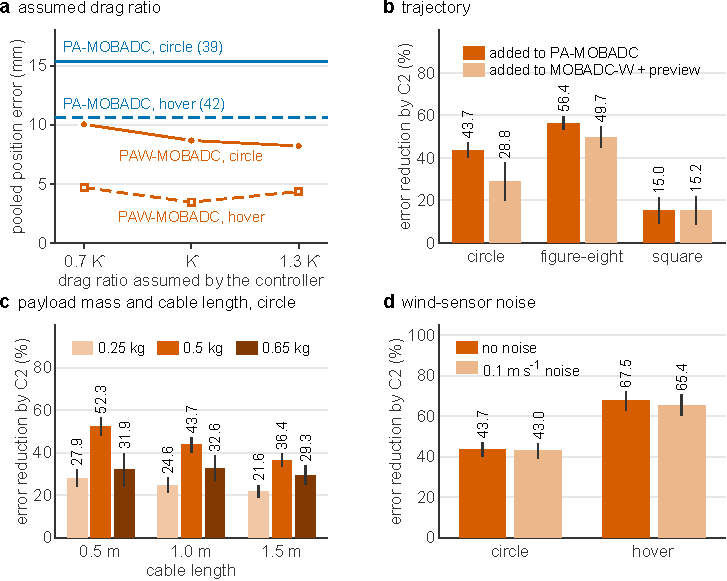
\includegraphics[width=\linewidth]{ijdc_sensitivity.pdf}
\caption{What the payload-drag term depends on, development sets: (a) pooled error against the drag ratio assumed by the controller (PA-MOBADC does not use it); (b) error reduction by C2 per trajectory, added to PA-MOBADC or to MOBADC-W + preview; (c) error reduction by C2 per payload mass and cable length on the circle; (d) error reduction by C2 with and without wind-sensor noise. Whiskers: \$\pm\$1.65 SE.}\label{fig:7}
\end{figure}


\begin{table}[!htbp]
\caption{What the payload-drag term depends on (development set, descriptive). $h = 1 -$ PAW-MOBADC / PA-MOBADC; in the preview rows the term is added to MOBADC-W + preview and $h = 1 -$ (PAW-MOBADC + preview) / (MOBADC-W + preview). ``1/day'' = one segment per day; ``unsat.'' = segments on which PA-MOBADC is below its tilt clamp.}\label{tab:c2}
\setlength{\tabcolsep}{3pt}
\begin{tabular}{@{}>{\raggedright\arraybackslash}p{0.34\linewidth}>{\raggedright\arraybackslash}p{0.2\linewidth}>{\raggedright\arraybackslash}p{0.18\linewidth}>{\raggedright\arraybackslash}p{0.18\linewidth}@{}}
\toprule
condition & development set & gain $h$ of the payload-drag term (SE) & complete controller / MOBADC-W $-$ 1 (SE) \\
\midrule
circle, nominal $\hat K$ & circle, 1/day & +43.67 \% (2.16) & $-$75.23 \% (1.05) \\
circle, $\hat K\times0.7$ & circle, 1/day & +34.76 \% (2.09) & -- \\
circle, $\hat K\times1.3$ & circle, 1/day & +46.70 \% (1.53) & -- \\
hover, nominal $\hat K$ & hover, 1/day & +67.51 \% (2.80) & -- \\
hover, $\hat K\times0.7$ & hover, 1/day & +55.81 \% (2.03) & -- \\
hover, $\hat K\times1.3$ & hover, 1/day & +59.00 \% (2.17) & -- \\
circle, wind-sensor noise 0.1 m/s & circle, 1/day & +42.98 \% (2.24) & -- \\
hover, wind-sensor noise 0.1 m/s & hover, 1/day & +65.36 \% (3.15) & -- \\
circle, spike filter on the measured wind & circle, unsat. & +38.00 \% (1.18) & -- \\
circle, no filter & circle, unsat. & +38.20 \% (1.21) & -- \\
hover, spike filter on the measured wind & hover, unsat. & +65.65 \% (1.62) & -- \\
hover, no filter & hover, unsat. & +65.68 \% (1.59) & -- \\
figure-eight & figure-eight & +56.37 \% (1.97) & $-$76.47 \% (0.69) \\
square & square & +15.03 \% (3.72) & $-$36.59 \% (1.02) \\
circle, $L$ = 0.5 m & circle, 1/day & +52.33 \% (2.50) & $-$80.32 \% (0.88) \\
circle, $L$ = 1.5 m & circle, 1/day & +36.43 \% (1.85) & $-$70.28 \% (1.06) \\
circle, $m_p$ = 0.25 kg & circle, 1/day, $U \le U_{\max}$ & +24.59 \% (2.14) & $-$53.96 \% (0.24) \\
circle, $m_p$ = 0.65 kg & circle, 1/day & +32.61 \% (3.59) & $-$69.50 \% (0.23) \\
circle, added to the preview & circle, 1/day & +28.80 \% (5.37) & $-$72.26 \% (0.39) \\
figure-eight, added to the preview & figure-eight & +49.73 \% (3.07) & $-$74.77 \% (0.57) \\
square, added to the preview & square & +15.25 \% (3.93) & $-$42.76 \% (0.42) \\
\botrule
\end{tabular}
\end{table}


\begin{itemize}
\tightlist
\item
  \emph{Assumed ratio.} With \(\hat K\) scaled by 0.7 and 1.3 the gain stays at 55.81 \% and 59.00 \% in hover (against 67.51 \% at the nominal ratio), and at 34.76 \% and 46.70 \% on the circle (against 43.67 \%). Underestimating the load's drag costs more than overestimating it, and neither removes most of the gain.
\item
  \emph{Swing and trajectory.} With the payload drag in the feed-forward the error falls by 56.37 \% on the figure-eight and by 15.03 \% on the square (development sets, PAW-MOBADC against PA-MOBADC). The square, whose corners excite the largest swing, is where the term helps least, as the swing-rate bound of Proposition 2 predicts.
\item
  \emph{Payload mass and cable length.} Across the eight sensitivity levels on the circle the gain lies between 21.64 \% (light payload, long cable) and 52.33 \% (short cable), and PAW-MOBADC lowers the error of MOBADC-W by 48.91 \% to 80.32 \%; the light-payload levels are pooled on the segments inside their wind envelope, as in Table~\ref{tab:sens}. The gain grows with the share of the load's drag in the wind force the vehicle has to balance.
\item
  \emph{Wind-sensor noise.} With 0.1 m/s noise on the wind sensor the gain is 42.98 \% on the circle and 65.36 \% in hover, against 43.67 \% and 67.51 \% without noise.
\item
  \emph{Reference preview.} Added to the preview instead of to the prediction, the payload-drag term lowers the error by 28.80 \% on the circle, 49.73 \% on the figure-eight and 15.25 \% on the square: C2 is independent of how the delay is compensated.
\end{itemize}

\subsection{Measurement versus prediction on the circle}\label{sec:measurement-versus-prediction-on-the-circle}

On the circle, where the payload force is periodic and fast compared with the loop delay, an acceleration-based estimate does not close the first gap. On the held-out days INDI-DE's pooled error is 37.2 mm, against 14.3 mm for PA-MOBADC and 8.73 mm for PAW-MOBADC (INDI-DE is 159.54 \% above PA-MOBADC; 112.93 \% on the development set; Fig.~\ref{fig:4}). Its error is nearly the same on every circle segment whatever the wind (Fig.~\ref{fig:6}a), and in the frame of the path it shows the same offset as MOBADC-W (Fig.~\ref{fig:5}): it measures the trajectory-driven payload force correctly and one loop delay late, the lag term of \eqref{eq:lag-err}. In hover, where the disturbance is slow, the comparison turns; Section~\ref{sec:when-to-predict-and-when-to-measure} discusses when measurement suffices.

\subsection{Advance knowledge of the wind (C3)}\label{sec:advance-knowledge-of-the-wind-c3}

Knowing the true future wind adds almost nothing once the wind is measured. In the registered headroom test the oracle lowered the error of PA-MOBADC by 0.69 \% on the circle and by 2.87 \% in hover with the wind-to-payload term (Fig.~\ref{fig:8}). The largest headroom among the eleven evaluable groups was 5.83 \% (a post-hoc group), below the registered threshold of 10 \%, so no group met the headroom rule. The residual error of PA-MOBADC therefore lies in the payload's response to the wind it already measures, which is what C2 addresses, and not in the timing of the wind.



\begin{figure}[!htbp]
\centering
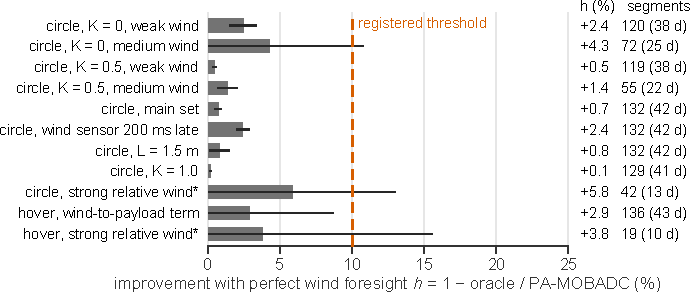
\includegraphics[width=\linewidth]{ijdc_oracle.pdf}
\caption{Error reduction from perfect advance knowledge of the wind, \(h\) = 1 \textminus{} oracle / PA-MOBADC, in the registered wind groups, with \$\pm\$1.65 SE; dashed: the registered threshold; right: \(h\), segments and days. *: post-hoc group. The group with strong wind on the circle at \(K = 0\) contained no segment.}\label{fig:8}
\end{figure}

\section{Discussion}\label{sec:discussion}



\subsection{When to predict and when to measure}\label{sec:when-to-predict-and-when-to-measure}

On the circle prediction wins (Section~\ref{sec:measurement-versus-prediction-on-the-circle}). \textbf{In hover}, where the disturbance is slow, fast measurement is enough: on the held-out days INDI-DE reaches 2.60 mm, against 3.85 mm for PAW-MOBADC and 10.6 mm for PA-MOBADC (Fig.~\ref{fig:9}). This advantage depends on the idealised accelerometer of Section~\ref{sec:actuators-and-sensors}. A horizontal accelerometer bias of 0.086 m/s$^2$ or 0.17 m/s$^2$, the gravity leakage of an attitude error of 0.50\textdegree{} or 0.99\textdegree{}, raises INDI-DE's error to 7.66 mm and 14.5 mm, above PAW-MOBADC, in agreement with the bias sensitivity of outer-loop INDI \cite{smeur2018}.


\begin{figure}[!htbp]
\centering
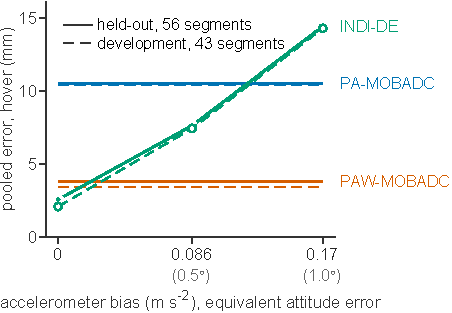
\includegraphics[width=\linewidth]{ijdc_measure.pdf}
\caption{Hover: pooled error of INDI-DE with a horizontal accelerometer bias, against PA-MOBADC and PAW-MOBADC, on the held-out days (solid) and on the development set with one segment per day (dashed). In brackets: the attitude error whose gravity leakage equals the bias.}\label{fig:9}
\end{figure}


The circle and hover results follow one rule: a disturbance that is periodic and fast compared with the loop delay has to be predicted, and a slow one can be measured. Prediction uses knowledge the controller already holds - the frequency in its internal model - and costs two trigonometric evaluations per mode; Proposition 1 guarantees that it does not amplify the observer's error. Measurement needs no model of the disturbance but arrives one delay late, which on a planned trajectory leaves the error that INDI-DE shows on the circle, and it inherits the accelerometer's bias, which removes its advantage in hover at an attitude error of half a degree. The view that disturbances cannot be predicted \cite{smeur2016} holds for disturbances without structure; a payload force on a planned path has structure that the observer has already identified.

\subsection{Two realisations of delay compensation}\label{sec:two-realisations-of-delay-compensation}

On a planned trajectory the loop delay can be compensated inside the observer (PA-MOBADC) or by feeding forward the reference acceleration one horizon ahead (MOBADC-W + preview). On the held-out days they give \textminus{}58.30 \% and \textminus{}62.40 \% against MOBADC-W, on the development set \textminus{}50.33 \% and \textminus{}53.95 \%; the two values differ by less than the standard error of either. Both need advance knowledge - the frequency of the payload force or the future trajectory - so neither applies to trajectories that are not planned. PAW-MOBADC uses prediction because it works inside the observer with the frequency the observer already holds and leaves the reference and the trajectory generator unchanged. The payload-drag term combines with either: added to the preview it lowers the error by 28.80 \% on the circle (Section~\ref{sec:c2-payload-drag-in-the-wind-feed-forward}).

\subsection{Limits of the payload-drag term}\label{sec:limits-of-the-payload-drag-term}

The term multiplies the measured airframe wind force by \(1+\hat K\), so its gain depends on the vehicle staying inside its actuator limits and on a clean wind measurement. On the full development hover set, including the segments where PA-MOBADC reaches its tilt clamp, the gain over PA-MOBADC is +20.27 \% (SE 42.39) instead of 65.68 \%: one segment at the actuator limit, on which both controllers saturate, dominates the pooled value (Table~\ref{tab:ablation}). This is why the held-out claim was registered on the segments below the tilt clamp; on the full held-out hover set the gain is 63.55 \%. The same multiplication passes measurement spikes to the force command: on one development segment of the circle and one of hover, both carrying single-sample spikes in the wind record, PAW-MOBADC stopped the solver while PA-MOBADC completed the run; none of the held-out segments produced a failure. A causal filter that holds a sample whose step exceeds 5 m/s did not remove these failures at no cost - it moved them to other segments, on two of which PA-MOBADC itself diverged with the filtered wind - and the gain was unchanged (38.00 \% on the circle and 65.65 \% in hover on the unsaturated segments, against 38.20 \% and 65.68 \% without the filter). A wind sensor for this term therefore needs spike handling designed with the controller, not a generic filter.

A richer model of the load does not help. Predicting the payload force with an open-loop pendulum model (MBP) did not pass its registered test: in hover it was worse than PA-MOBADC on the full set (\(h\) = \textminus{}158.83 \%, SE 200.46), although better on the unsaturated segments (+72.72 \%), and on the circle its error was 222.33 \% above PA-MOBADC. A model of the load that runs open loop diverges from the real swing, whereas the static term of C2 and the observer of C1 both stay tied to measurements.

\subsection{What advance wind knowledge can add}\label{sec:what-advance-wind-knowledge-can-add}

For the 61--74 m wind of this dataset the measured-wind channel is already close to the oracle: the sensor delay is one sample, and the static drag model passes the low-frequency wind that dominates the force. The error that remains is the payload's own dynamics, which C1 and C2 address. Wind nearer the ground carries more energy at high frequency and may leave more headroom for prediction. On the unsaturated segments of one post-hoc group, strong hover wind relative to the envelope, the oracle gained 41.52 \% (10 development segments); the held-out days held a single usable segment in that wind band, so H-hover was not confirmable.

\subsection{Control effort and payload swing}\label{sec:control-effort-and-payload-swing}

The lower error costs control effort. On the held-out days the RMS oscillation of the rotor forces of PAW-MOBADC is 0.611 N on the circle, against 0.532 N for MOBADC, 0.579 N for PA-MOBADC and 0.543 N for INDI-DE, and 0.556 N in hover, against 0.532 N for PA-MOBADC and 0.503 N for INDI-DE. On the circle this is about 15 \% more effort than MOBADC for a 78 \% lower position error. The method improves the position of the vehicle, not the swing of the load: the payload's RMS angle is almost the same for every controller, 16.24--16.88\textdegree{} on the circle, where it is mostly the steady cone angle of about 15\textdegree{}, and 7.99--8.03\textdegree{} in hover. Damping the swing calls for feedback of the cable angle \cite{sreenath2013}.

\subsection{The boundedness assumption and the published gains}\label{sec:the-boundedness-assumption-and-the-published-gains}

Section~\ref{sec:boundedness-of-the-closed-loop} rests on a baseline that is input-to-state stable with respect to its compensation error. With Guo's gains \cite{guo2020} the full plant stayed stable on all ten registered runs at a motor lag of 17 ms and diverged on all ten at 25 ms and at 30 ms. Guo et al.~flew these gains stably \cite{guo2020}; a motor lag of 17 ms is consistent with that and is used throughout. The result agrees with the observation that position and attitude gains are not free once actuator dynamics are taken into account \cite{smeur2018}, and it marks where the boundedness assumption holds for this baseline.

\subsection{Scope}\label{sec:scope}

The results are simulation results, and the comparisons are designed so that the conclusions do not depend on favourable modelling: the accelerometer is ideal, which favours the acceleration-based competitor; the competitor's filter is the best value of a sweep; and the baseline's published gains are used unchanged. Results hold for planned trajectories and hover. The held-out days had entered pooled wind statistics of an earlier stage of the project, and the two days inspected there in detail were removed before any controller run; the held-out confirmations rest on fourteen days.

\section{Conclusion}\label{sec:conclusion}

On a quadrotor with a slung load in measured wind, the error that remains under an observer-based controller with a wind measurement is set by two model gaps, and both can be closed with knowledge the controller already has. Propagating the payload estimate over the loop delay through the observer's exosystem lowers the error of the measured-wind controller by 58 \% on fourteen held-out days, and adding the payload's drag to the wind feed-forward lowers it by a further 63 \% in hover and 37 \% on the circle; both steps were registered and confirmed on the held-out days, the second after being found on development data. The complete controller, PAW-MOBADC, lowers the error of the multiple-observer controller of Guo et al.~on the circle by 78 \% at about 15 \% higher control effort, and neither addition can destabilise a baseline that is input-to-state stable with respect to its compensation error.

For practitioners:

\begin{enumerate}
\tightlist
\item
  Compensate the loop delay for a periodic payload force: predict the observer's estimate through its exosystem, or preview the planned reference (\textminus{}58 \% and \textminus{}62 \% on the held-out days).
\item
  Put the payload's drag into the wind feed-forward; an assumed drag ratio 30 \% too low or too high keeps most of the gain.
\item
  Expect little from predicting the wind at 61--74 m height: perfect foresight gained at most 6 \% in any wind group.
\item
  Use an acceleration-based estimate for slow disturbances in hover only if the attitude error is well below 0.5\textdegree{}.
\item
  Check published gains against the motor lag of the platform: the baseline gains are stable at 17 ms and diverge from 25 ms.
\end{enumerate}

Flight tests, wind measured near the ground, and swing damping are the next steps.

\backmatter

\bmhead{Data availability}
The wind records are public data of the M5 tower of the NREL National Wind Technology Center (https://wind.nlr.gov/MetData/135mData/M5Twr/). The simulation and analysis code will be made publicly available on GitHub upon acceptance; the registers and the result files will be made available upon acceptance.

\bmhead{Declarations}
Competing interests, funding and the authors' contributions are stated on the separate title page (double-anonymous review); the use of AI-assisted tools is described in Section~\ref{sec:use-of-ai-assisted-tools}.

\begin{appendices}

\section{Components added to the simulation model}\label{sec:components-added-to-the-simulation-model}

Every component that this work adds to the simulation model of the baseline is inserted by one named script, and nothing else in the model is. Inherited from Guo et al., unchanged: the rigid-body model, the attitude and position laws with every gain, the position and attitude observers, the disturbance observer with its one-harmonic exosystem, and the composition of \eqref{eq:guo-law}.


\begin{center}\footnotesize
\begin{tabular}{@{}p{0.46\linewidth}p{0.22\linewidth}p{0.22\linewidth}@{}}
\toprule
\textbf{component} & \textbf{inserted by} & \textbf{used in this paper} \\
\midrule
plant P2 (spherical pendulum, quadratic drag, motor lag, sensors, discrete loops), the controller's quadratic wind model with its \((1+\hat K)\) scale, the INDI-DE and MBP blocks, the wind-to-payload term of C3 and the known-weight trim & \texttt{build\_p2\_plant} & yes - Sections~\ref{sec:model}, \ref{sec:measured-wind-feed-forward}--\ref{sec:comparison-methods} \\
DC mode of the observer's internal model & \texttt{build\_do\_matrices} & yes - MOBADC-DC and every variant after it \\
payload predictor \(\boldsymbol B e^{\boldsymbol A\tau}\hat{\boldsymbol\xi}\) & \texttt{build\_payload\_predictor} & yes - C1 \\
measured-wind path into \(\hat{\boldsymbol d}_{lf}\) (made quadratic through \texttt{build\_p2\_plant}) & \texttt{build\_pa\_mobadc} & yes - MOBADC-W \\
reference preview \(\ddot{\boldsymbol\gamma}_d(t+\tau_{prev})\) & \texttt{build\_traj\_preview} & yes - MOBADC-W + preview \\
trajectory shapes (hover, circle, figure-eight, square, multi-sine) & \texttt{build\_traj5} & yes \\
measured wind series & \texttt{build\_wind\_series} & yes \\
frozen learned wind predictor & \texttt{build\_wind\_predictor} & C3 only \\
wind-sensor noise injection & \texttt{build\_wind\_sensor\_noise} & Section~\ref{sec:c2-payload-drag-in-the-wind-feed-forward} (0.1 m/s) only \\
inactive blocks kept from an earlier version of the model, switched off in every run & \texttt{build\_payload\_pendulum}, \texttt{build\_payload\_wind}, \texttt{build\_payload\_inject}, \texttt{build\_im\_est\_online} & no \\
probes on the wind estimate and on the vehicle acceleration & \texttt{build\_dlf\_probe}, \texttt{build\_nu\_dot\_log} & instrumentation only \\
tilt, thrust, rotor and torque limits & \texttt{thrust\_attitude\_ref}, \texttt{motor\_allocation} & yes - Section~\ref{sec:actuators-and-sensors} \\
\botrule
\end{tabular}
\end{center}


\end{appendices}

\bibliographystyle{sn-nature}
\bibliography{references}

\end{document}
